\newpage
\section{Подсистема журналирования}

Подсистема журналирования в Системе администрирования ЛПУ предоставляет удобный интерфейс для просмотра лога событий, зарегистрированных в ФТМИС.

Для организации ведения журнала событий необходимо:
\begin{enumerate}
 \item Установить систему журналирования;
 \item Включить журналирование событий в ФТМИС;
 \item Указать адрес системы журналирования в Системе администрирования ЛПУ.
\end{enumerate}
 
Пункты 1-2 описаны в документации к соответствующим системам.

Для настройки работы подсистемы журналирования в Системе администрирования ЛПУ необходимо нажать кнопку \btn{Журнал}  на панели управления и в открывшейся странице нажать кнопку \btn{Настройки}. Откроется страница настроек данной подсистемы (Рисунок \ref{img_jur_conf}).

\begin{figure}[ht]\centering
 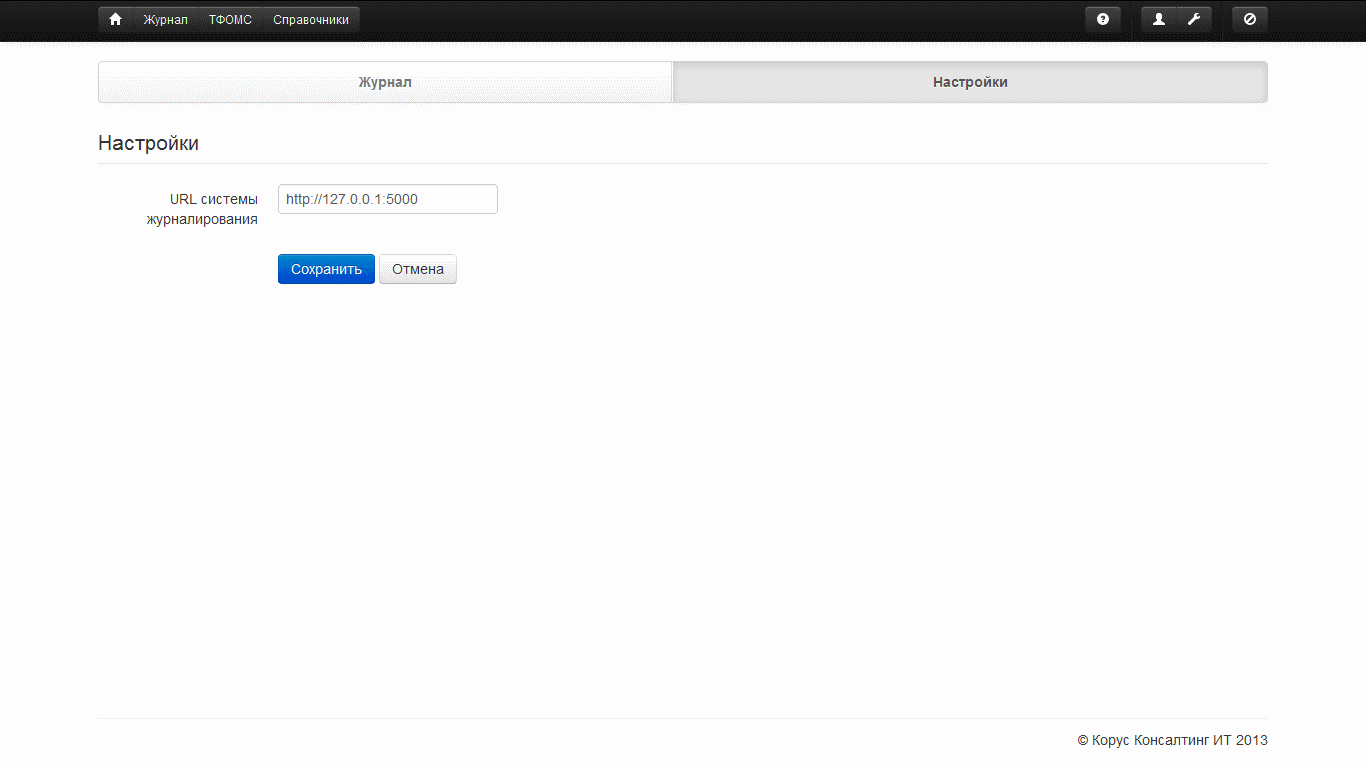
\includegraphics[width = 1\textwidth ,keepaspectratio]{jur_conf}
 \caption{Настройка подсистемы журналирования}
 \label{img_jur_conf}
\end{figure}

В поле \dm{URL системы журналирования} следует ввести адрес, по которому доступна система журналирования, а затем сохранить изменения, нажав кнопку \btn{Сохранить}.